\chapter{Introduction}\label{chapter:introduction}

\begin{comment}Dead kitten: since the first CS degrees were awarded in the late 1960s
\footnote{Some CS departments are considering or already implementing course enrollment limits, which may disproportionately affect underrepresented students \cite{personalconversationwithjasonchuang}.}
Enrollment in computer science, including programming classes, has been growing. We are now experiencing a third boom in student interest \cite{csBoom}.
\end{comment} 

Given growing demand, programming class sizes at major universities like MIT, Stanford, Berkeley, and University of Washington are reaching hundreds or thousands of students. However, one-on-one tutoring is considered a gold standard for the educational outcomes it regularly produces \cite{bloom}. The rapid, personalized feedback and attention that is possible within a one-on-one tutoring relationship or a small class becomes prohibitively difficult or expensive at larger scales. Systems and techniques that scale the benefits of low student-to-teacher ratios to arbitrarily many students is an on-going challenge in modern education.

Computers are a natural ally in this challenge. Even though computers do not yet have a human's ability to design curriculum, compose an entirely new question, or handle a novel answer, their attention, computation, and memory scales much better than humanity's. This thesis work supports a vision of teaching computer science education where humans--teachers and students--are front and center, discussing approaches, design choices, and trade-offs, augmented by computation behind the scenes.

The challenge of scaling up computer science education is usually framed as simply coping with the problems of large class sizes. This thesis, however, explores how the volume of students and their solutions can be exploited to enable new types of rapid personalized feedback, as well as recover aspects of a traditional small class.

Learners individually solving programming or digital hardware design problems can collectively generate a wide variety of possible bugs and solutions. A single programming or digital hardware design exercise may yield thousands of student solutions that vary in many ways, some superficial and some fundamental. For teachers, this variation can, for example, be a source of pedagogically valuable examples and corner cases that slipped past an automatic grader. For students, the variation in a large class means that other students may have struggled along a similar solution path, hit the same bugs, and can offer hints based on that earned expertise. 

Understanding large-scale variation in student solutions requires identifying appropriate features of solutions, developing ways to automatically extract those features from each solution, user interface design to communicate the results to teachers or students, and possibly the collection of additional information from students through learnersourcing. This thesis includes the development of four systems that take advantage of the solution variation in large classes. All four systems have been evaluated using data or live deployments in on-campus or edX courses with hundreds or thousands of students.

\section{A Tale of Two Turing Machines}

This work began after midnight in the basement computer lab of the Stata Center, where a student was struggling to create a Turing Machine that could detect whether a string of open and closed parentheses was properly balanced. If he was not successful within the next day or two, he would fail Computer Architecture (6.004). I will refer to him as Paul. I had a hard time helping Paul turn his Turing machine into one that would pass all the automatic grader's test tapes. I could not tell if his approach could work with a little debugging or was fatally flawed. I did not want to demoralize him by telling him to abandon his efforts so far and start over unless it was truly necessary. And what if he was on the path to a novel solution no one else had created before?

While not a necessary condition for the correctness of his intended approach, finding a similar working solution in the pool of previous student submissions would serve as an existence proof and evidence that he should persevere. I had copies of hundreds of other students' correct Turing machines, but it was difficult to see by inspection whether any of these solutions were successful implementations of his intended approach. This was due to both superficial static and dynamic differences between solutions. There are two sources of static superficial differences: (1) students design their own symbol library and state names for the finite state machine portion of their Turing machine (2) students can list behavioral specifications in terms of their custom symbol and state names in any arbitrary order. Each behavior-specifying rule is a computer-readable version of the form ``if you're in state X and you read symbol Y on the tape, overwrite symbol Y with symbol Z, move the tape-reader in direction W, and transition to state Q." Dynamic superficial differences arise because even after translating these textual statements into a finite state machine diagram, the diagrams look very different from one correct solution to the next.

Eventually, through trial and error, he got his Turing Machine to work on all the test tapes, and passed the course. But I was deeply troubled by the experience. I felt like the information was there, in our staff server, but my brain could not see through the superficial textual differences nor mentally execute all the student solutions I had access to in order to have the perspective that would have helped me help Paul, when I could not see the bugs in his Turing Machine directly.

After the semester ended, I looked into this further. I ran all the correct two-state Turing machines collected during the semester on the same test tape containing a string of open and closed parentheses. The movement of the tape-reading head across this input was logged in coordinates relative to the common starting point, at the left end of the test tape, and displayed along the vertical axis. The horizontal axis represents the number of steps taken by the Turing machine on its way to completing the task. These discrete steps are analogous to time. 

The majority (88\%) of the solutions employ one of two mutually exclusive strategies. These strategies were identified just from visual inspection of the movement of many Turing machines across the common test tape. Figure \ref{turingFig} shows their locations on the common input tape over time, separated by strategy into Figures \ref{tapeMoveA} and \ref{tapeMoveB}. These two strategies for determining whether or not the tape's string of parentheses is balanced are (1) matching the innermost open parenthesis with the innermost closed parenthesis, i.e., standard semantic interpretation in math, and (2) matching the $n^{th}$ \todo{fix this font} open parenthesis with the $n^{th}$ closed parenthesis. The remaining 12\% of solutions (not shown) include less common strategies. This analysis also exposes room for improvement in the suite of test tapes: at least two strategies in this group are known to pass the test tapes but are actually incorrect because they cannot handle an arbitrary depth of nested parentheses. 

%Each staff member is encouraged to complete the Turing Machine lab on their own before counseling students. 
Staff members were aware of the Turing machine solution they each had found on their own time, and yet were not aware that there were two mutually exclusive common solutions. At least one staff member admitted steering students away from solutions they did not recognize, but in retrospect may have indeed been valid solutions. 

Based on my analysis, I was able to brief fellow 6.004 staff members on the space of solutions--both good and bad--in preparation for subsequent semesters and could suggest additions to the test tape suite to catch submissions that were previously erroneously marked as correct. 

This experience was a critical and formative one for me. It has inspired the design approach and technical approach taken in many of the systems that follow.

\begin{figure*}[p]

\begin{subfigure}[b]{1.0\textwidth}
\centering

\includegraphics[width=140mm]{Body/figures/ICERtapeLocations.png}
\caption{Tape on which all 148 two-state Turing machines were tested, and the numbering system by which locations along the test tape are identified.}
\label{tapeLocations}
\end{subfigure}

\begin{subfigure}[b]{1.0\textwidth}
\centering
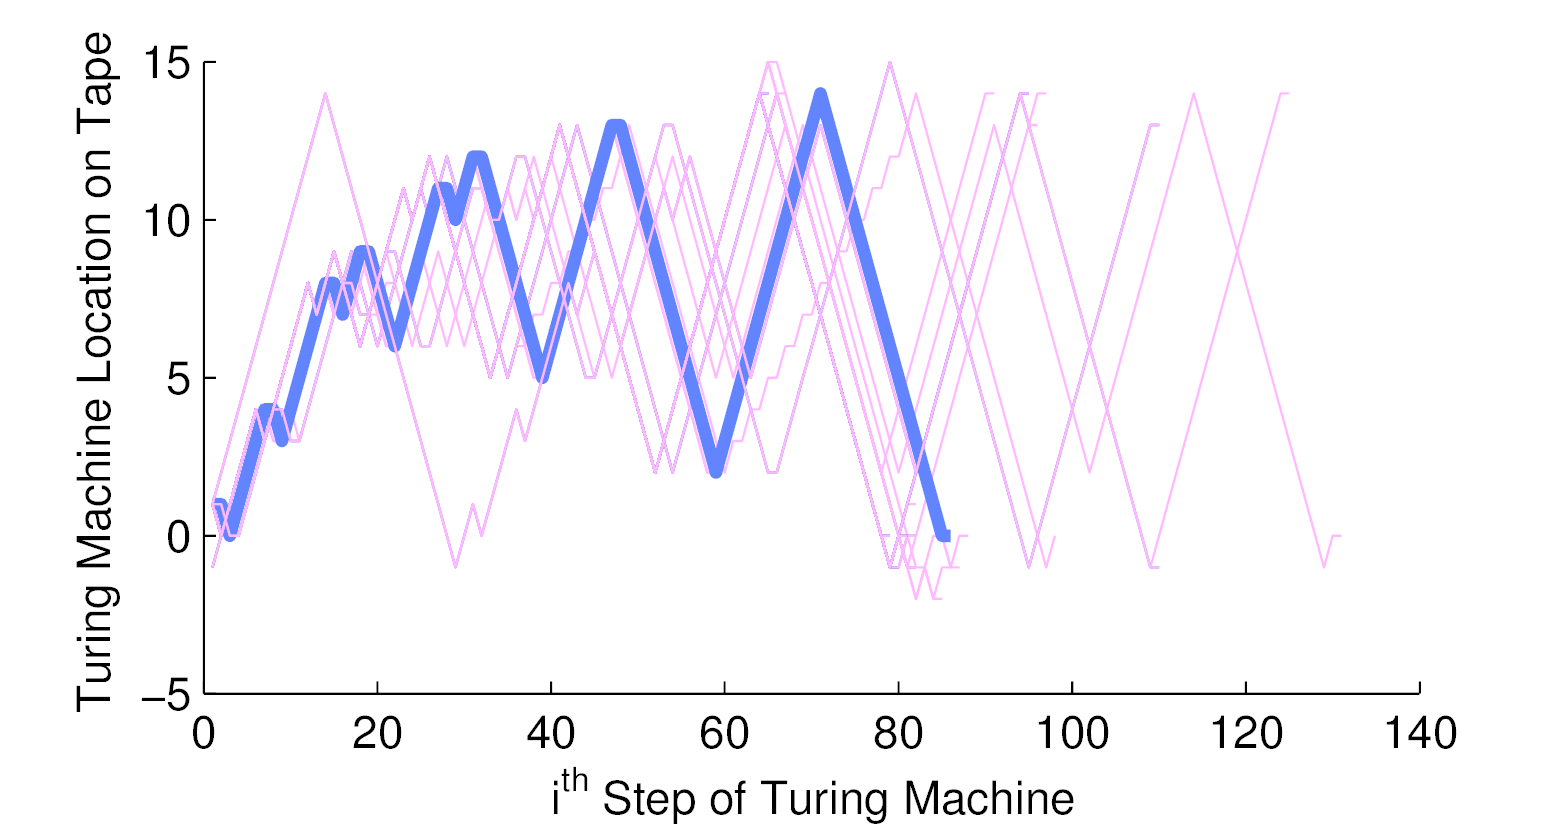
\includegraphics[width=0.85\textwidth]{Body/figures/tmvisualization_InnerParensMatched_allkidsAnno2}
\caption{Strategy A Turing machines: those which paired inner sets of open and closed parentheses, as is standard in mathematical notation. (73 out of 148 Turing machines)}
\label{tapeMoveA}
\end{subfigure}

\begin{subfigure}[b]{1.0\textwidth}
\centering
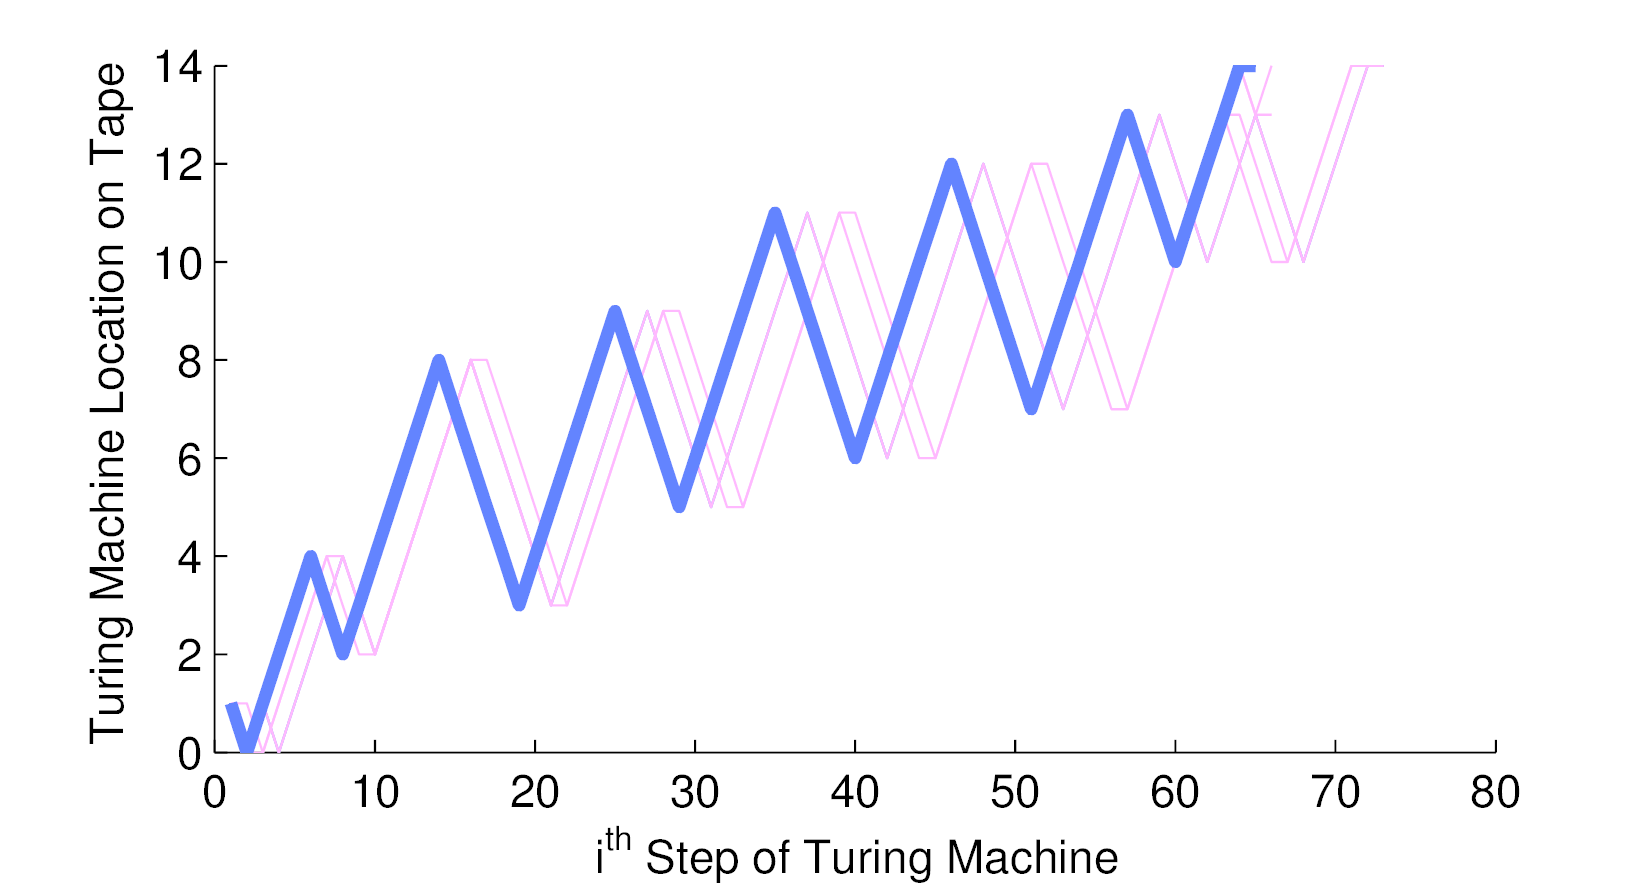
\includegraphics[width=0.85\textwidth]{Body/figures/tmvisualization_NtoNParensMatched_allkidsAnno2}
\caption{Strategy B Turing machines: those which paired the first open with the first closed parenthesis, the second open with the second closed parenthesis, etc. (58 out of 148 Turing machines)}
\label{tapeMoveB}
\end{subfigure}

% \begin{subfigure}[b]{1.0\textwidth}
% \includegraphics[scale=0.85]{Body/figures/tmvisualization_Other_allkidsAnno}
% \caption{The trajectories of the 17 remaining Turing machines, run on the same common test tape as above, which have yet to be categorized. Both bold trajectories correspond to solutions that do not work in general, but passed the provided, fixed test suite.}
% \label{tapeMoveC}
% \end{subfigure}

\caption{The two most common strategies for a two-state Turing machine to determine if a string of parentheses is balanced. Figures \ref{tapeMoveA} and \ref{tapeMoveB} show tape head position over time on the tape illustrated in Fig. \ref{tapeLocations}. The bold trajectories represent particularly clean examples.}
\label{turingFig}
\end{figure*}



\section{OverCode}

In MOOCs, a single programming exercise may produce thousands of solutions from learners. Understanding solution variation is important for providing appropriate feedback to students at scale. The wide variation among these solutions can be a source of pedagogically valuable examples, and can be used to refine the autograder for the exercise by exposing corner cases. We developed OverCode to visualize and explore thousands of small Python programs that solve the same problem. OverCode uses both static and dynamic analysis to cluster similar solutions, and lets teachers further filter and cluster solutions based on different criteria. We evaluated OverCode against a non-clustering baseline in a within-subjects study with 24 teaching assistants, and found that the OverCode interface allows teachers to more quickly develop a high-level view of student understanding and misconceptions, and to provide feedback that is relevant to more student solutions.


\begin{figure}
\centering
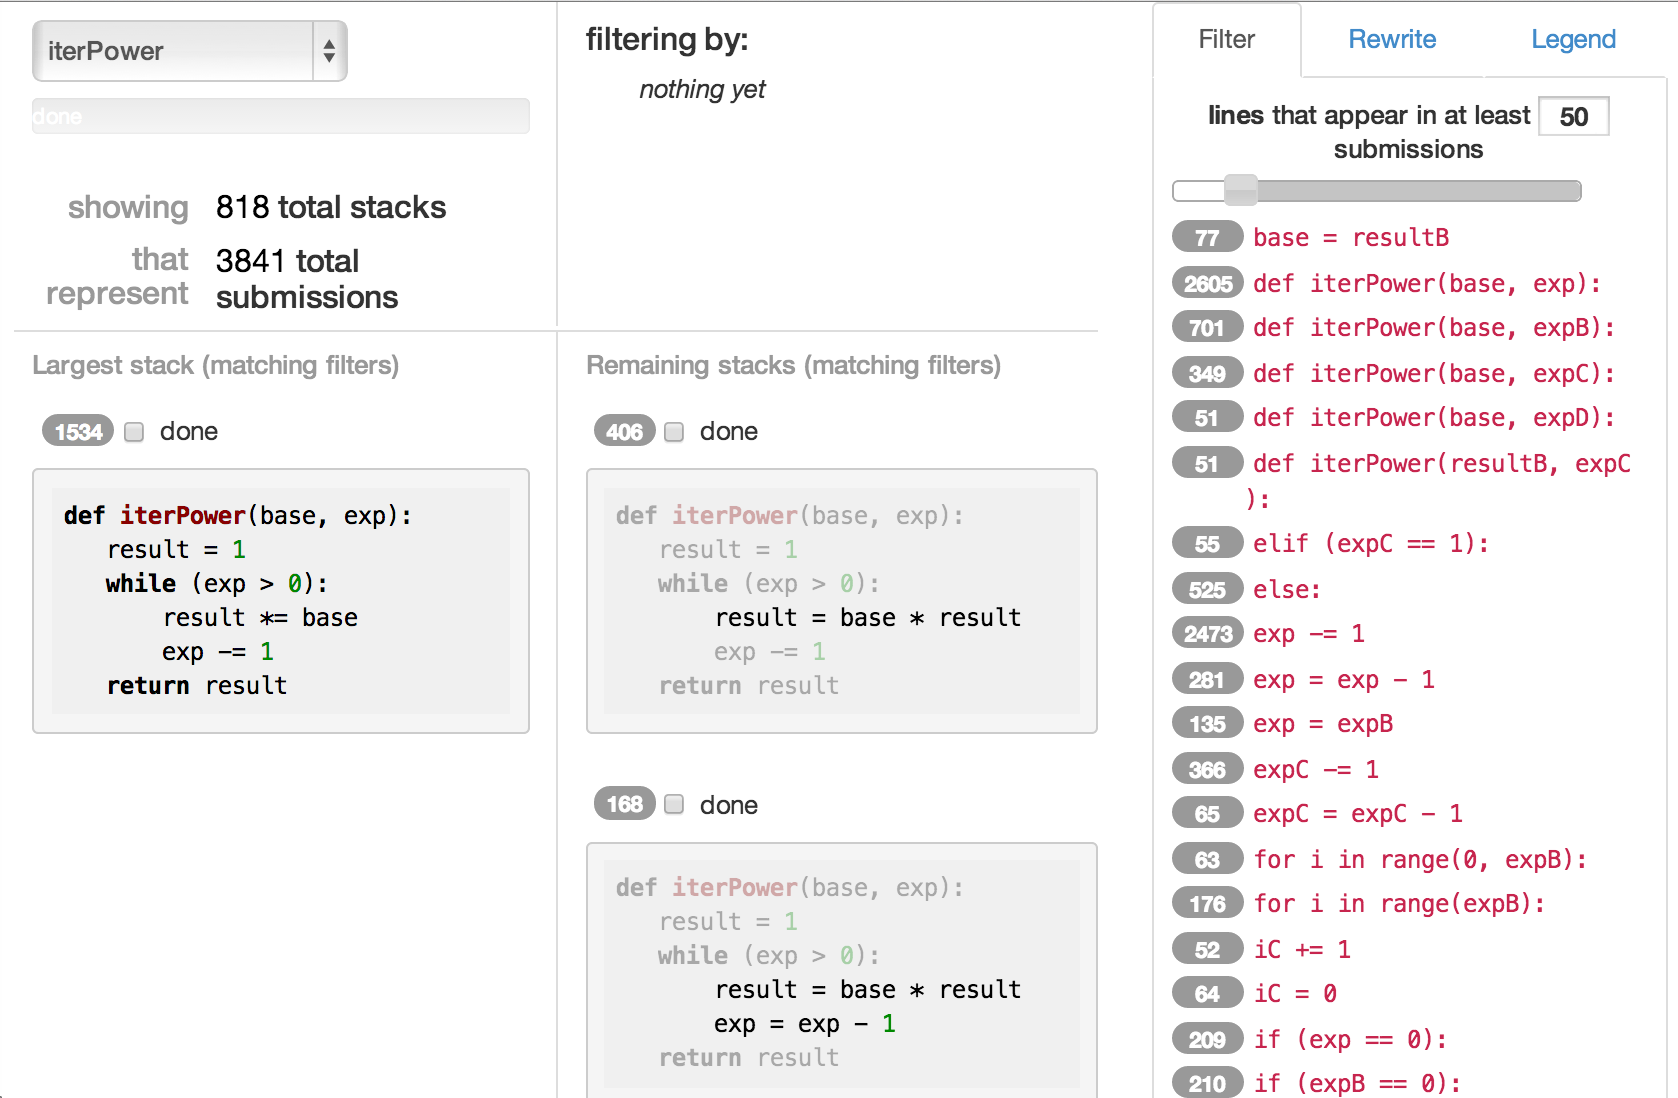
\includegraphics[width=1.0\linewidth]{Body/figures/interfaceScreenShot.png}
\caption{The OverCode user interface. The top left panel shows the number of clusters, called {\it stacks}, and the total number of solutions visualized. The next panel down in the first column shows the largest stack, while the second column shows the remaining stacks. The third column shows the lines of code occurring in the cleaned solutions of the stacks together with their frequencies.}
\label{fullinterface}
\end{figure}


\section{Foobaz}

Traditional feedback methods, such as hand-grading student code for substance and style, are labor intensive and do not scale. We created a new user interface that addresses feedback at scale for a particular and important aspect of code quality: variable names (see Figure \ref{fig:figure2}). Foobaz distinguishes variables by their behavior in the program, allowing teachers to comment not only on poor names, but also on names that mislead the reader about the variable's role. We ran two lab studies of Foobaz, one with teachers and the other with students. In the first study, 10 Python teachers used Foobaz to comment on variable names in thousands of student solutions from an introductory programming MOOC. In the second study, 6 students composed fresh solutions to the same programming problems, and immediately received personalized variable-name quizzes composed in the previous user study.

\begin{figure}
	\centering
	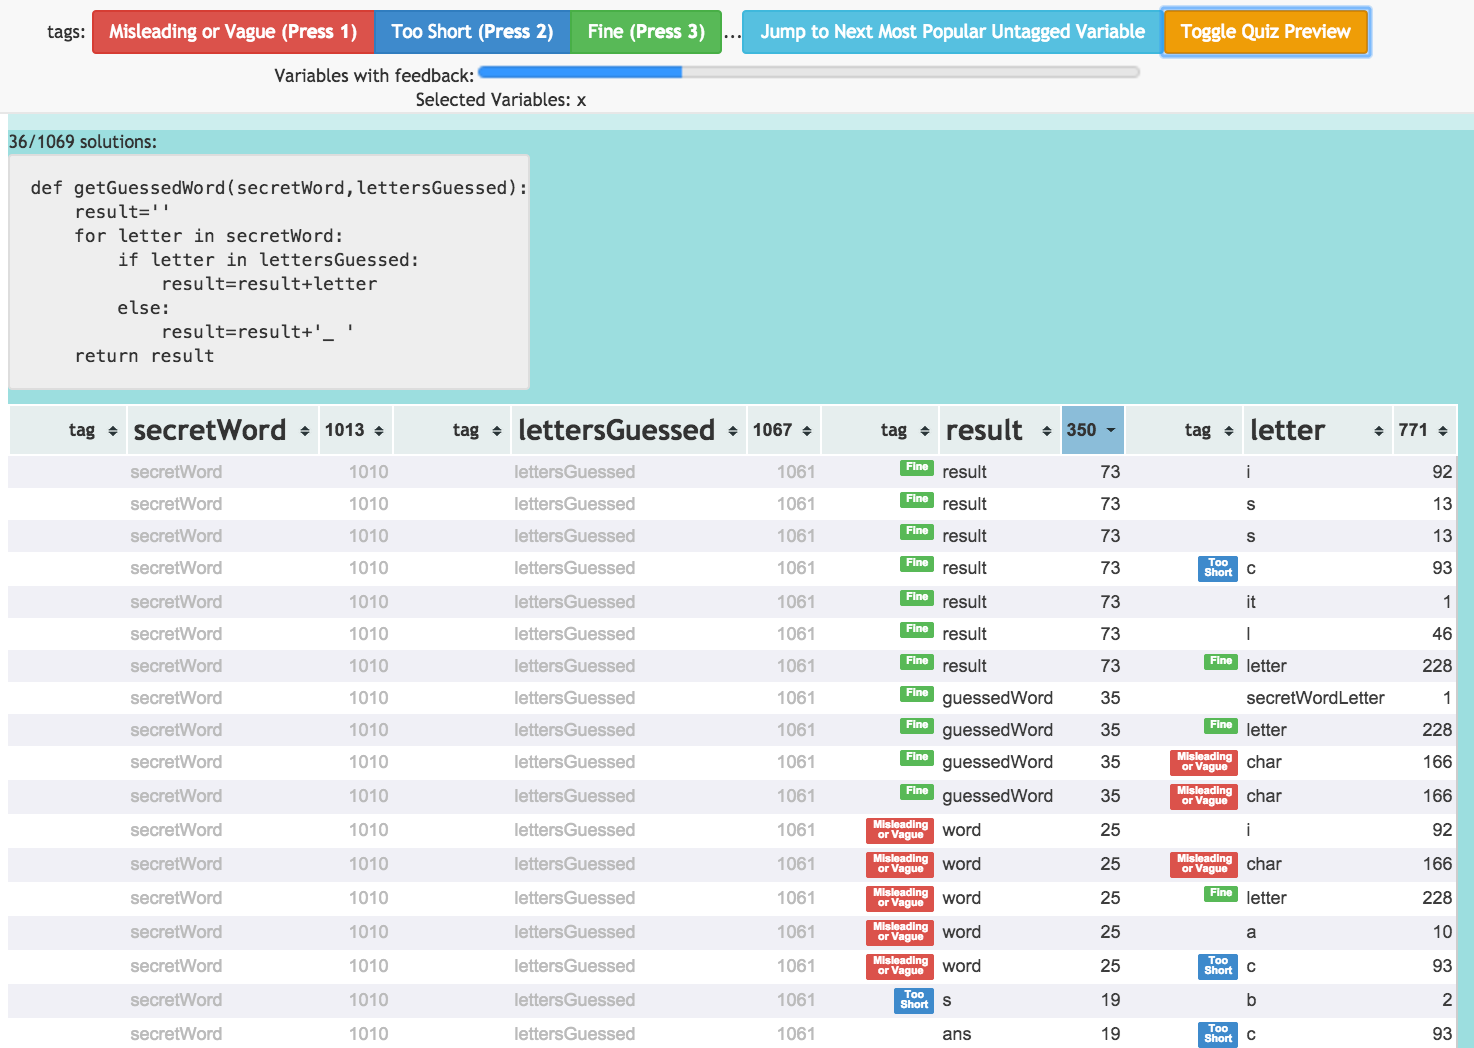
\includegraphics[width=1.0\linewidth]{Body/figures/FoobazInitialFat.png}
	\caption{The Foobaz teacher interface. The teacher is presented with a scrollable list of normalized solutions, each followed by a table of student-chosen variable names. Some names shown here have been labeled by the teacher as ``misleading or vague,'' ``too short,'' or ``fine.''}
	\label{fig:figure2}
\end{figure}

\todo{include the student view}

\section{Extensions of OverCode Clustering}

In order to perform more comprehensive clustering, several extensions of the original OverCode clustering methods have been explored and some have been fully implemented.
GroverCode is an extension of OverCode built to canonicalize and cluster both correct and incorrect solutions. This was also done in the context of hundreds of exam-level solutions instead of thousands of solutions to "finger exercises" and problem set problems. This change in regime was inspired by need-finding interviews with the lecturer who teaches both the online and residential versions of MIT's introductory Python programming class. She was appreciative of the insights OverCode could give her extracted from the thousands of correct solutions submitted by her online students, but the semi-regular pain of hand-grading the hundreds of incorrect solutions submitted by tuition-paying residential students was a more immediate concern. Adapting to the needs of a team of graders grading a smaller number of more complex solutions, many of which were incorrect, required significant changes to the pipeline and interface. The resulting system was deployed to the staff for use during two grading sessions. The results of this field deployment are also promising; the staff welcomes its continued use in future semesters. More preliminary explorations of statistical methods for clustering solutions are also described.

\section{ClassOverflow}

Personalized support for students is a gold standard in education, but it scales poorly with the number of students. Prior work on \textit{learnersourcing} presented an approach for learners to engage in human computation tasks while trying to learn a new skill. Our key insight is that students, through their own experience struggling with a particular problem, can become experts on the particular optimizations they implement or bugs they resolve. The students can then generate hints for fellow students based on their new expertise. ClassOverflow  uses new workflows to harvest and organize students' collective knowledge and advice for helping fellow novices through design problems in engineering (see Figure \ref{fig:workflow}). ClassOverflow was evaluated in an undergraduate digital hardware design class with hundreds of students. We show that, given our design choices, students can create helpful hints for their peers that augment or even replace teachers' personalized assistance, especially when that assistance is not available.


\begin{figure}
\centering
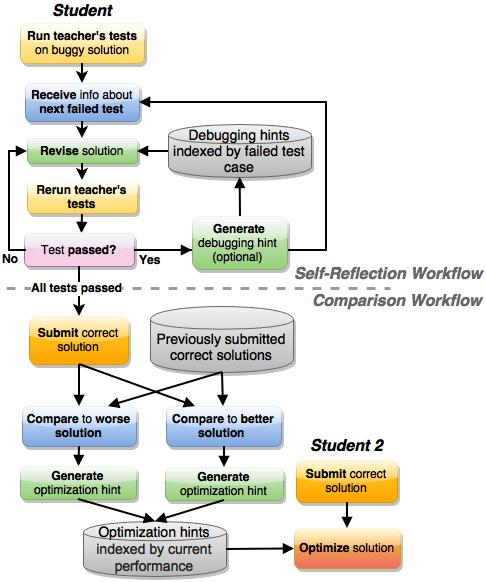
\includegraphics[width=1.0\linewidth]{Body/figures/classoverflow/CombinedWorkflow_CameraReady_FIXED_2.jpg}
\caption{In the \textit{self-reflection} workflow, students generate hints by reflecting on an obstacle they themselves have recently overcome. In the \textit{comparison} workflow, students compare their own solutions to those of other students, generating a hint as a byproduct of explaining how one might get from one solution to the other.}
\label{fig:workflow}
\end{figure}




\begin{comment}
\section{Discussion}
Learnersourcing has been a recurring topic at CSCW recently, and these systems show various mechanisms for leveraging learners in large engineering classes. Learners produce many variations of solutions to a problem, running into common and uncommon bugs along the way. Learners can be part of a closed system workflow that prompts them to generate analysis of their own activity and sends it to selected fellow learners as feedback. Alternatively, learners can be pure producers whose activity is analyzed by systems and distilled by teachers into personalized feedback for fellow learners. We would like to demo these systems together, as a suite of learnersourcing systems that allow teachers to turn the challenges of teaching at scale into an opportunity for discussion, self-reflection, peer-teaching, and more learning from examples.
\end{comment}

\todo{block-quote this}
{\bf My thesis statement is: Clustering and visualizing solution variation collected from programming courses can help teachers gain insights into student design choices, detect autograder failures, award partial credit, use targeted learnersourcing \todo{make sure targeted learnersourcing is defined} to collect hints for other students, and give personalized style feedback at scale.}

\section{Terminology}

\todo{Finish defining: solutions, programming exercise/problem, collections of solutions to an exercise....}

Since terminology across research domains can vary, I will define the terms in which I will describe previous research and my own: 
\begin{itemize}
\item A {\it solution} is code that a particular person wrote in response to a prompt or problem description.
\item {\it Solution clusters} represent different patterns of implementation. For example, there may be two distinct solution clusters, both achieving the same input-output behavior but by different means. \todo{better name for this, that respects topic model approach?}
\item A {\it solution path} is a series of code snapshots generated while a person is working toward meeting a particular input-output behavior specification. 
\item The {\it space of student solutions} refers to the aggregation of student-generated solutions and the solution clusters they form.
\item {\it Learnersourcing}... \todo{define, using my own wording if necessary}
\end{itemize}

\section{Contributions}

\todo{add grovercode contributions, turn into prose}The main contributions of this thesis are:
\begin{itemize}
\item A novel visualization that shows similarity and variation among thousands of Python solutions, with cleaned code shown for each variant. 
\item An algorithm that uses the behavior of variables to help cluster Python solutions and generate the cleaned code for each cluster of solutions.
\item Two user studies that show this visualization is useful for giving teachers a birds-eye view of thousands of students' Python solutions.
\item A technique for displaying clusters of Python solutions with only a slice of each cluster exposed, revealing the features that are relevant to the task. In this application, the relevant features are variable names and roles.
\item A workflow for generating personalized active learning exercises, emulating how a teacher might socratically discuss good and bad choices with a student while they review the student's solution together.
\item A working system which implements the above technique and method for datasets from both MOOCs and large residential classes on introductory Python programming.
\item Two lab studies which evaluate both the teachers' and students' experience of the variable name feedback workflow.
\item{A self-reflection learnersourcing workflow in which students generate hints for each other by reflecting on an obstacle they themselves have recently overcome while debugging their solution to a Python or digital design exercise.}
\item{A comparison learnersourcing workflow in which students generate design hints for each other by comparing their own solutions to alternative designs submitted by other students.} 
\item{A deployment of the self-reflection workflow in a 200-student class and a lab study of the comparison workflow with 9 participants. Results from these studies show that personalized hints can be viably learnersourced, and that these hints serve as helpful guides to fellow students encountering the same obstacle or attempting to reach the same goal.}
\end{itemize}

\section{Thesis Overview}

Chapter \ref{chapter:relatedwork} summarizes prior and contemporary relevant research on systems that support programming education. It also briefly explains theories from the learning sciences and psychology literature that influenced or support the pedagogical value of the design choices made within this thesis.

The four chapters that follow describe, in detail, the four systems developed, as well as their evaluation on archived data or in the field.

\begin{itemize}
\item OverCode (Chapter \ref{chapter:overcode}) visualizes thousands of programming solutions using static and dynamic analysis to cluster similar solutions. It lets teachers quickly develop a high-level view of student understanding and misconceptions and provide feedback that is relevant to many student solutions. 

\item Foobaz (Chapter \ref{chapter:foobaz}) clusters variables in student programs by their names and behavior so that teachers can give feedback on variable naming. Rather than requiring the teacher to comment on thousands of students individually, Foobaz generates personalized quizzes that help students evaluate their own names by comparing them with good and bad names from other students. 

\item ClassOverflow (Chapter \ref{chapter:classoverflow}) collects and organizes solution hints indexed by the autograder test that failed or a performance characteristic like size or speed. It helps students reflect on their debugging or optimization process, generates hints that can help other students with the same problem, and could potentially bootstrap an intelligent tutor tailored to the problem.

\item OverCode Extensions (Chapter \ref{chapter:grovercode}) describes (1) GroverCode, an extension to OverCode optimized for processing and displaying incorrect as well as correct student submissions and (2) clustering and mixture modeling algorithms applied to the OverCode pipeline's output for additional insight into patterns within student solutions. %The GroverCode user interface is optimized and deployed in the field for teachers awarding partial credit to each of the hundreds of students who submitted programs in computer-based quizzes and final exams for the residential Python-based introductory programming (6.0001) and data science (6.0002) courses at MIT.
\end{itemize}

Chapter \ref{chapter:discussion} discusses the design lessons that apply to the entire collection of systems in this thesis. Chapter \ref{chapter:futurework} outlines avenues of future work this thesis work, in combination with the complementary work of others in this space, paves the way for.



\begin{comment}"one-on-one tutoring promotes both greater student learning and increased student motivation to learn compared with traditional, formal classroom teaching and learning settings" --http://www.ncbi.nlm.nih.gov/pmc/articles/PMC3292071/ \end{comment}


\begin{comment}

Dead kittens:

In introductory programming and digital circuit design education, this thesis aims to change the traditional curve in the quality of education as a function of class size from monotonically decreasing to a U-shape. As a proxy for measuring learning outcomes, the systems developed in this thesis empower old or entirely new rapid, personalized feedback modes similar to those delivered in a one-on-one teaching relationship but enabled by the scale of students composing solutions to class exercises.

By second grade, children should be able to write simple, coherent stories \cite{http://www.webmd.com/parenting/features/when-should-kids-learn-read-write-math}. 

When I was much younger, my dad taught me about vacuum tubes. With few modifications, tubes can serve as amplifiers, switches, or displays. ``Tube: The Invention of Television'' tells the dramatic history behind the invention and commericialization of the first televisions, which were built with cathode ray tubes. At critical parts of the story, he'd ask, e.g., ``How you would change the intensity of the electron beam hitting the screen?'' just before the authors were about to reveal how the inventors would get past their next technological hurdle.

Sometimes, I had no idea how to answer. Sometimes, I came up with something similar to what the inventors came up with. And sometimes, because I was not biased by the actual scientific literature that the inventors were immersed in, I came up with something very different, but possibly also effective. 

The systems in this thesis help teachers take advantage of the massive collections of solutions, enabling either (1) the same teaching practices that were previously only tractable in smaller courses or (2) new practices that are only possible when a massive collection of student solutions are available.

This thesis describes several systems designed to (1)  (2) (3) amplify teachers' actions, by enabling them to compose and deliver personalized feedback to more students while expending minimal additional effort. 

Despite recent advances in artificial intelligence, human and computer intelligence remain largely complementary. Humans can compose new questions and handle novel answers, while computers can perform prescribed analyses of thousands of student answers orders of magnitude faster than humans. 

Ways of delivering the rapid, personalized feedback that  commonly accepted practices of good teaching d

As enrollment in programming courses grows, some teaching practices and systems may become prohibitively expensive or arduous to use.

This thesis documents several novel tools I developed for helping hundreds or thousands of students learn how to program. The demand for programming education is growing rapidly, and this thesis treats the volume of students in programming classes not as a problem, but as an opportunity. It begins with the story of how I learned to program, and ends with a description of new tools for teachers and students engaged in the hard work of transferring the knowledge and practice of programming from one generation to the next.

At heart, I'm an electrical engineer, and it has informed my approach through-out. To me, a class of students is a system I want closed-loop control over: with the control policy of an experienced teacher and knowledge of the state of the system--my hundreds or thousands of students--I can better steer it to my intended destination of knowledge and skills.

I similarly think of solutions as systems that turn inputs into outputs, sometimes in the same way, sometimes in different ways.
\end{comment}
